\graphicspath{{figures/design/}}
\chapter{Test Journal: rocket motor test}\label{ThrusterTest}
\label{ssc:ThrusterTest}
\begin{table}[!h]
\begin{tabular}{l l}
\textbf{Test participants:} & Raphaël  \\
\textbf{Date:}  & 31/03-2017
\end{tabular}
\end{table}

\section*{Purpose}
The purpose of this test is to characterize the thrust of the Klima D3-P rocket motor.
\section*{Test equipment and components}
\begin{table}[h]
	\centering
	\caption{List of measurement equipment and components}\label{tab_appendix:SRB_equip}

	\begin{tabularx}{\textwidth}{lXXXX}
		Name 				& Brand	& Model & AAU-number									\\ \toprule \rowcolor{lightGrey}
		Torsion scale	& Made in AAU & N/A & N/A 	\\
		Rocket motor	& Klima &  D3-P & N/A \\ \rowcolor{lightGrey}
		3D printed adapter & N/A & N/A & N/A
	\end{tabularx}
\end{table}
\section*{Setup}
Measurement setup is seen on \autoref{fig:DCSetup} \
\begin{figure} [h]
\centering
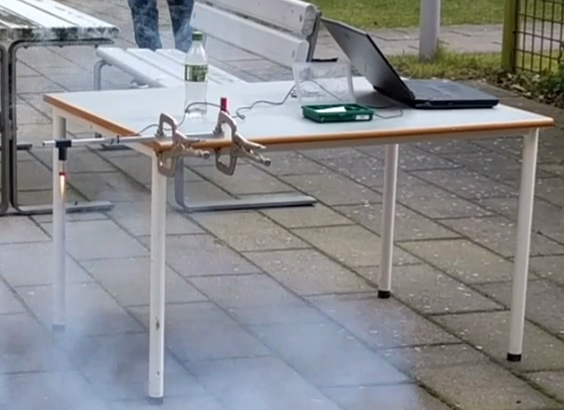
\includegraphics[width=0.8\linewidth]{figures/appendix/srb_test_setup.png}
\caption{Measurement setup.}
\label{fig:SRBSetup}
\end{figure}

The torsion scale was lent by Jens Frederik Dalsgaard Nielsen, and the Arduino code was improved to filter the data. This code is available in the attached files.

\section*{Method}
The scale was calibrated using a known weight before the experiments.

\begin{enumerate}
\item The motor is placed inside the adapter, facing the ground
\item The scale is clampled strongly on the table. The clamping should be the same as during the calibration.
\item Scale turned on, a standard quick fuse and a lighter was used to start the motor.
\item After the motor had burned, the scale was shut off and the files on its SD card copied to a computer.
\item The operation was repeated with two motors from two different boxes.
\item Using Matlab, the data was plotted and put to scale according to the calibration.
\end{enumerate}
\section*{Raw data}
The raw data from the scale is in the attached files.
\section*{Data processing}
Using the calibration weight, the data was put to scale using the Matlab code "scale_reader.m" attached. It produced the graph displayed here. The force in Newton was translated in equivalent gram of lift for easier interpretation.

\begin{figure} [h]
	\centering
	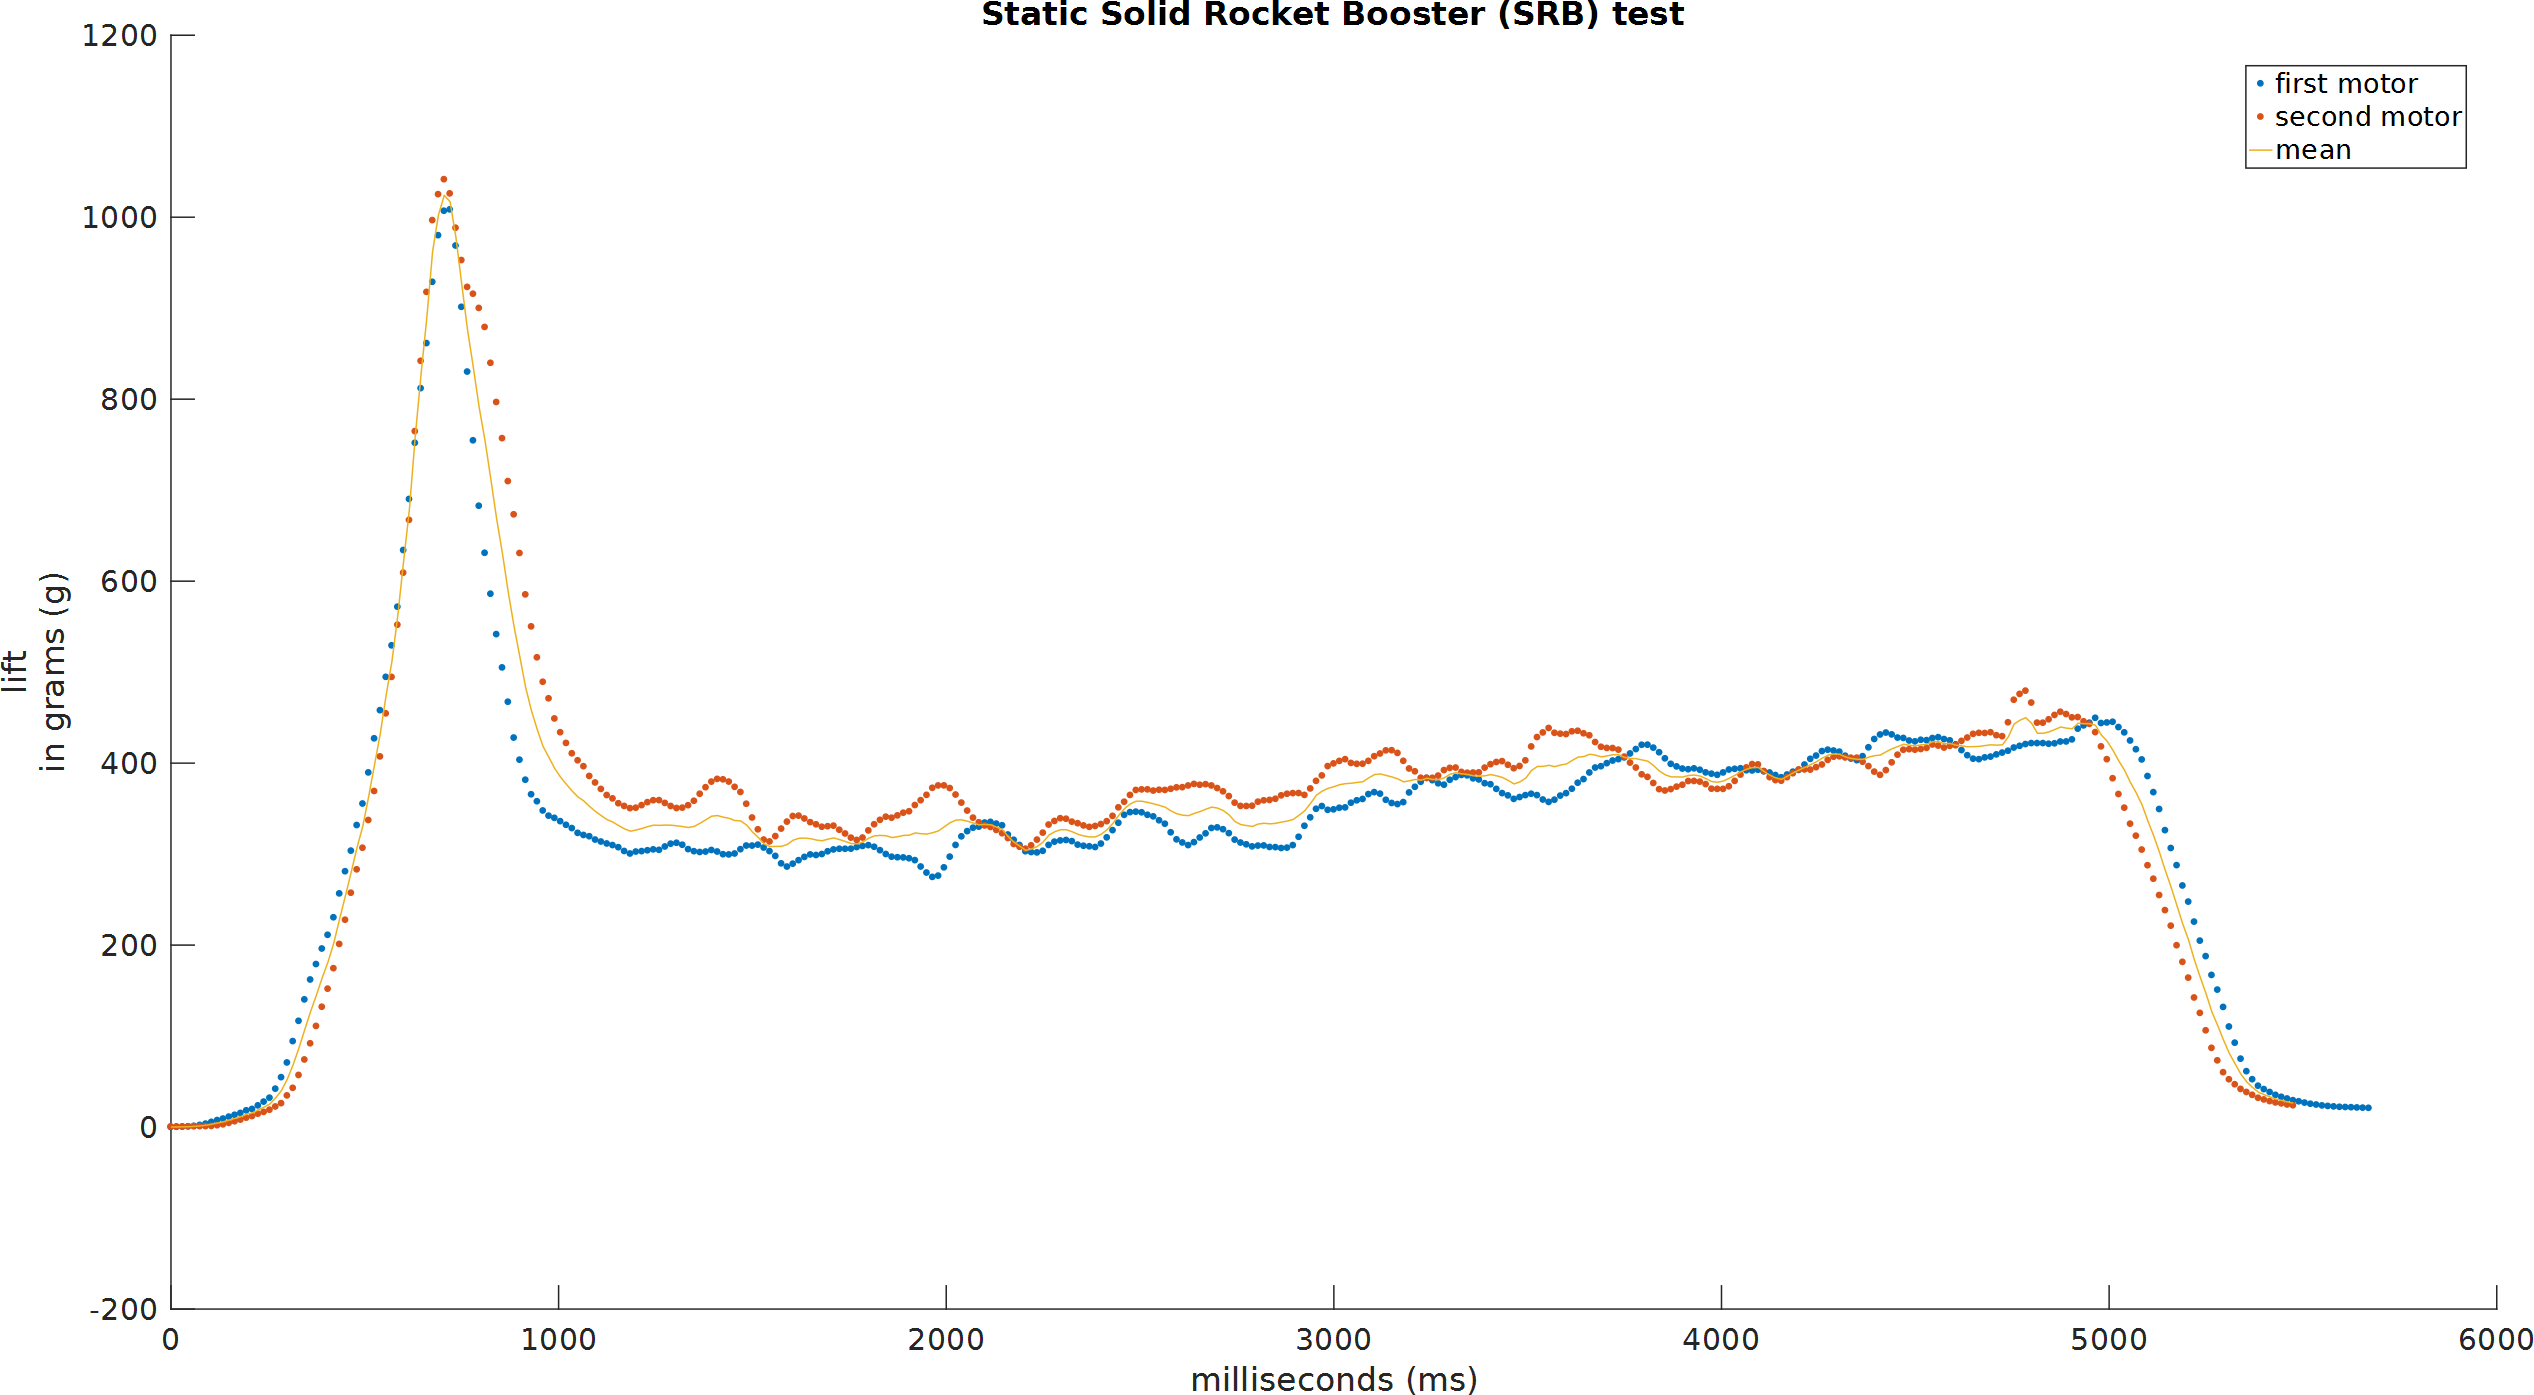
\includegraphics[width=\linewidth]{figures/appendix/srb_test}
	\caption{Processed thrust data}
	\label{fig:thrust_graph}
\end{figure}

\section*{Conclusion}
It can be seen that the two motors are very similar. The thrust builds up quickly producing a force peak of around 10 Newtons, or 1 Kg equivalent lift, for less than 400 ms. It then goes down and stabilizes to 330 grams of lift, slowly going up to 410g (taking in account the 20g mass loss of the motor during the thrust). Since the rocket is less than 300 grams, the motor should be able to lift it.


